\chapter{Courses 2 LMS}



Now, that we have understaning of how CodeIgniter works, we can continue with description of Courses 2 system, as it was developed by Jakub Culiks work \cite{culik}. Motivation of this chapter is to describe this system as it was implemented before this work, explain motivation for creating a new learning management system (LMS) and bring some technical details of Courses 2 LMS. This chapter is considered as an introduction to our work and may be used to differentiate our work from previous works.

\section{Motivation}

Courses 2 system was developed during spring and winter of 2015 with development team led by Jakub Culik. This team was able to create a simple, customizable and modular learning management system which is already used at our faculty. Until the end of summer semester of 2016, 32 courses with total of 200 students were using this system.


Need for this system started in 2010, when a new aproach of the learning was introduced in the web design course at our faculty \cite{culik}. Each student had to publish a multiple blog posts which where then evaluated by his classmates and teachers of the course. Ratings were then projected into his final grade from this course. This approach led students to study more about topics they were interested in and were related to this subject. With this approach, students were also forced to discuss these problems and got greater insight into blog topics.


Used blog portal \texttt{blog.matfyz.sk} was also developed at our faculty in 2008 by Martin Rejda \cite{rejda}, so there were many options improve this system and to modify it to our needs. For example, blog portal was modified to allow students to implement and submit their own blog layout in XSLT. Hovewer, there were still some missing features like system for reviewing of these blog articles and discussions so the need for another system arose \cite{culik}. As a solution, new system, Courses was created \cite{culikbc}.


This system was developed as a part of bachelor's thesis in 2013 \cite{culikbc} and was running 4 courses for one year \cite{culik}. After this time, it seemed clear that this system has to be completely redesigned and implemented from scratch. A new system had to be modular, scalable and well designed. And so, Courses 2 was born.

\section{Semantics}

Courses 2 system architecture can be divided into two parts: system part and modules. This division is required for maintaining this system modular and scalable. Now, let's look at each part.

\subsection{System}

System part is mostly responsible for "background stuff". Models and controllers extend standard CodeIgniter classes and there is only a few standalone libraries. All files of this part are located in \texttt{application/} folder and comply with standard CodeIgniter MVC flow. All libraries of system part are loaded once on each request.


Main goal of this part is to share all data to every component. For example, after user login, user information have to be avaible for each module. Since Course and Layout information are shared too, it is placed here as well. This part is also responsible to decide which modules has to be run on specific request and printing their outputs on the correct place in application layout.

\subsection{Modules}

After system initialized all required classes, correct modules has to be run. Currently, there are 5 modules installed: \texttt{Core}, \texttt{Assignments}, \texttt{Quiz}, \texttt{Notes}, \texttt{Results}. Each module has different purpose and we will later explain \texttt{Assignments} throughoutly as it is main focus of this work. Other modules work similar and are not referenced by us, so we do not consider their description important for this work. It can, hovewer, be found in previous works \cite{culik}.

\subsection{Layout}

Layout is managed by system part of this application. CodeIgniter default layout system is not sufficient for modularity, so it had to be replaced by a new one. Main problem was that each part of layout can be rendered by different module, which is decided at run-time. So page structure was divided into 4 different parts, each with its own rendering.


Courses 2 is build to offer one, root layout for all of the pages. It is not needed to create multiple different layouts in learning management system such as this. So there is just one, root layout, which is located in \texttt{application/views} directory of the project. This layout can be easily changed but this is not main focus of this work.

\begin{figure}[h]
    \centering
    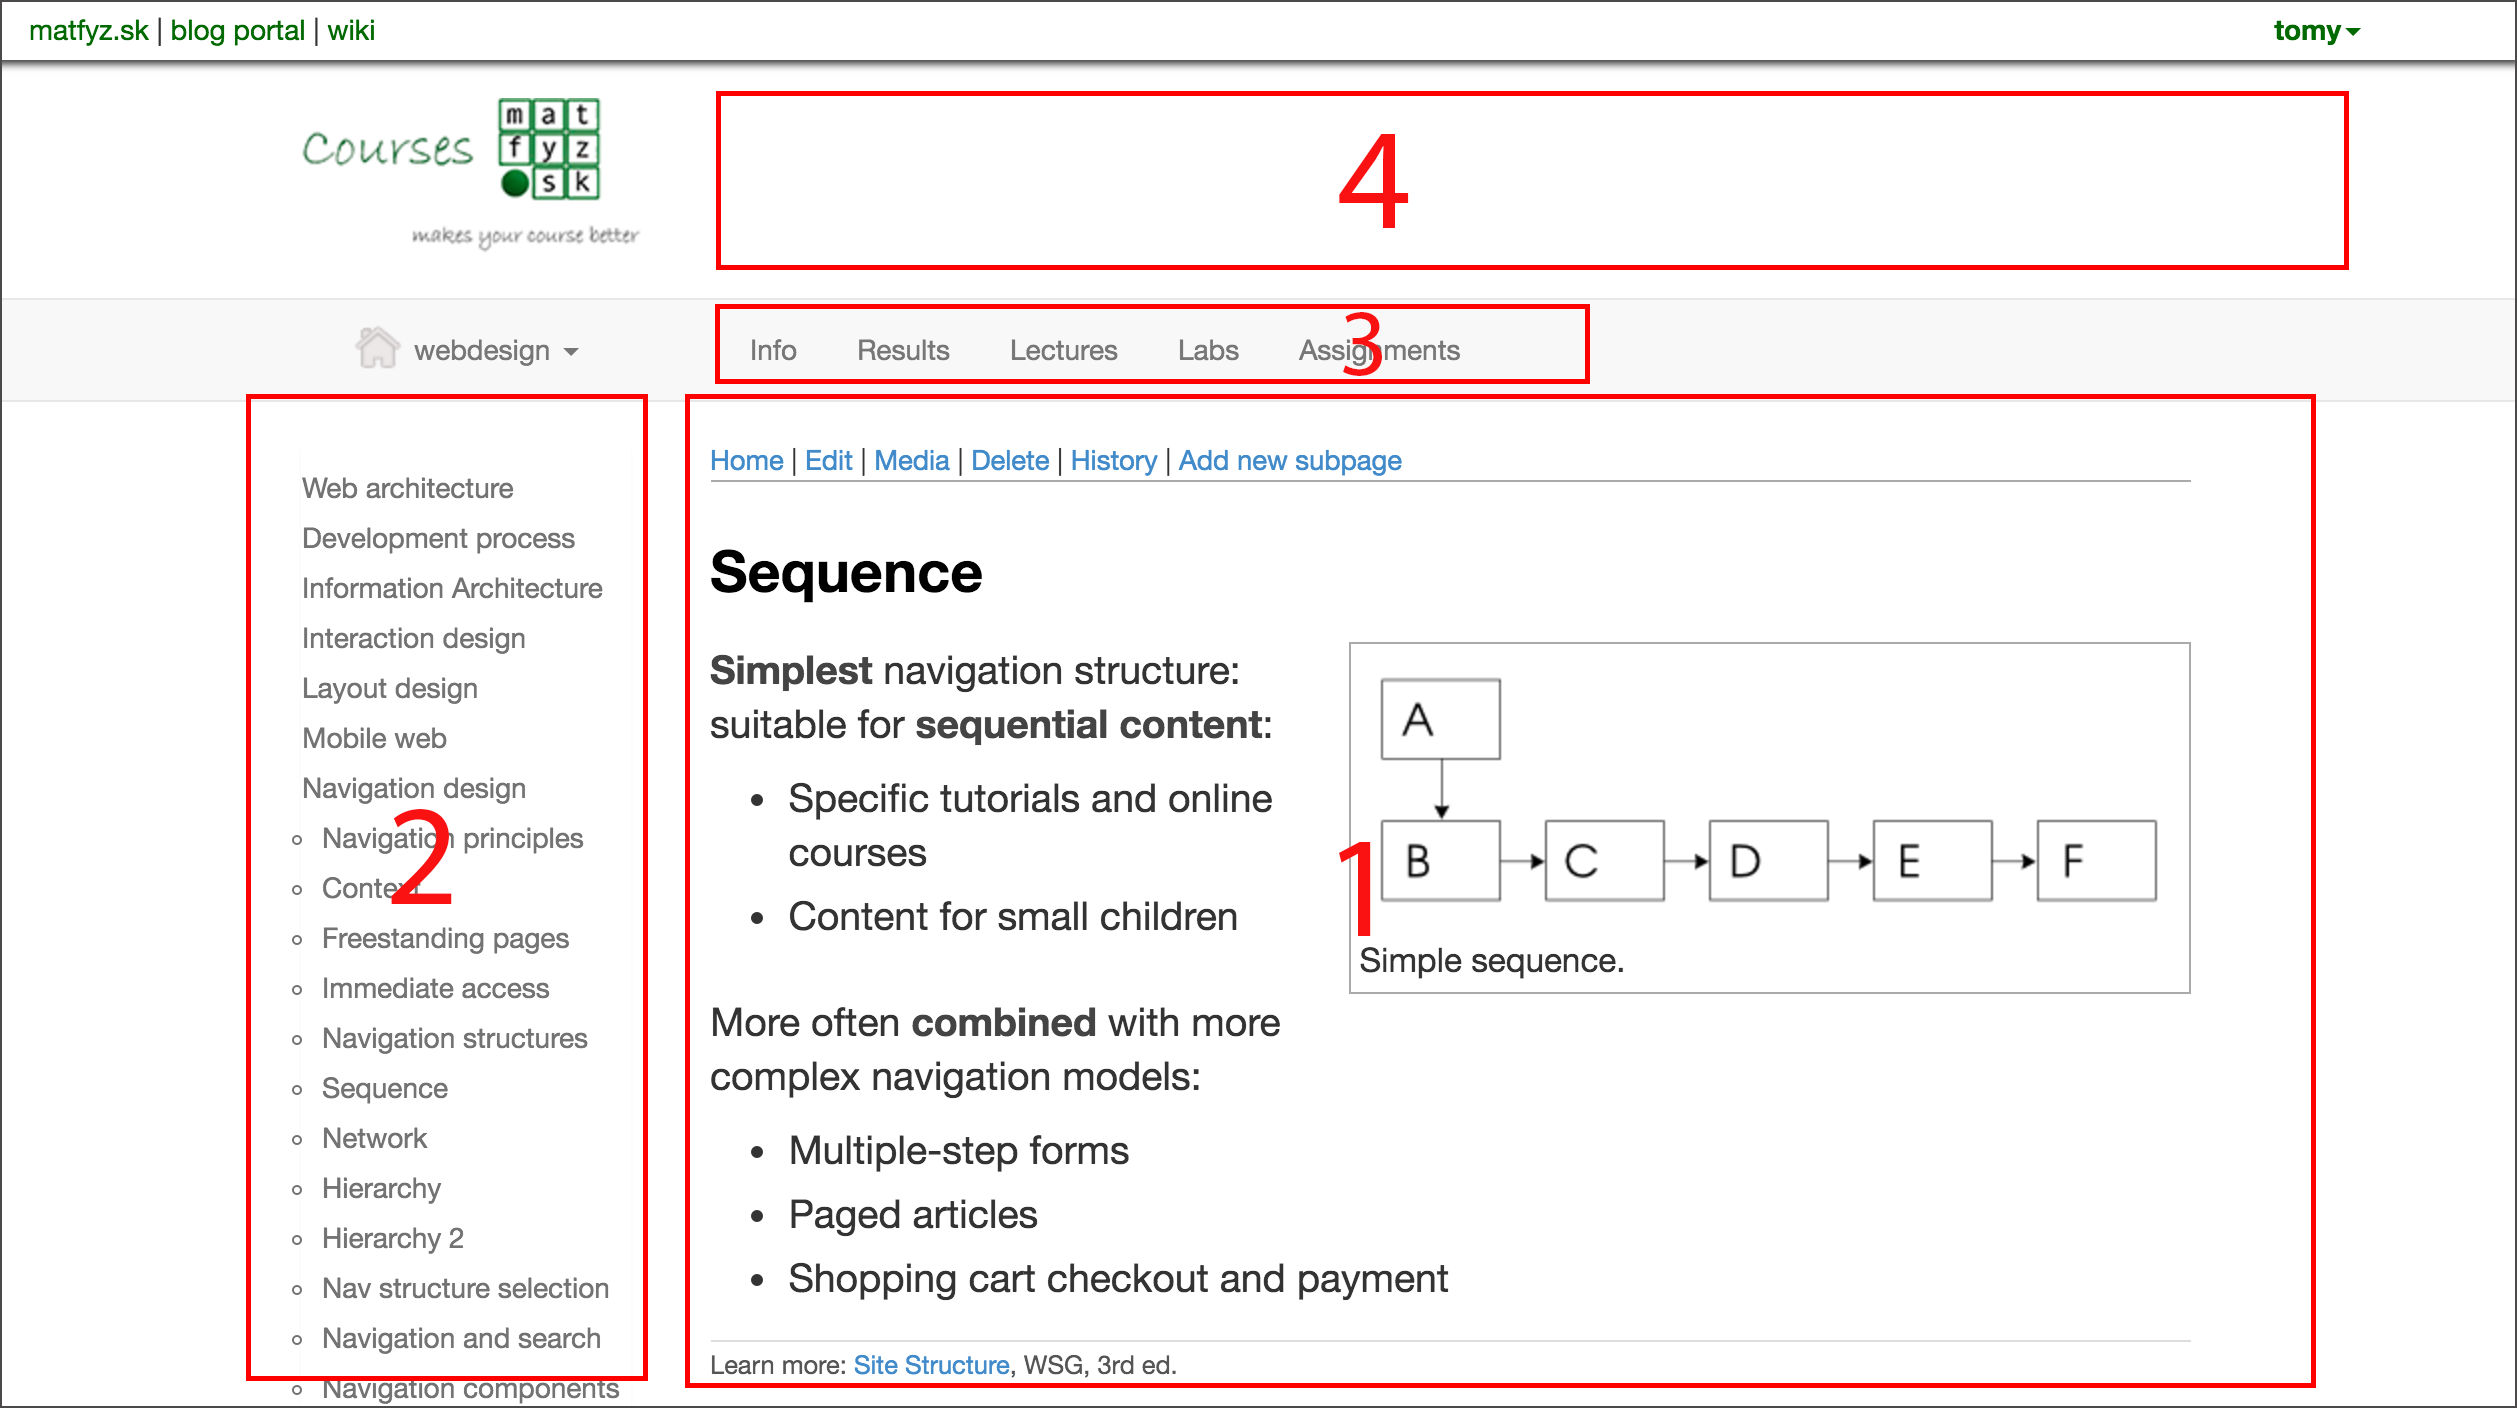
\includegraphics[width=0.95\textwidth]{images/courses-labelled.png}
    \caption{Courses 2 screenshot}
    \label{courses2screen}
\end{figure}


As we can see on figure \ref{courses2screen}, root layout was split into 4 different parts, each with specific purpose and rendered independently. Each numbered part is rendered by selected module, the rest is rendered by system. This screenshot was rendered using \texttt{Notes} module as it is showing content of a lecture. Part number 4 is reserved for notifications, such as new assignment was created or so.

\section{HMVC extension}

Now, let's focus on hierarchical model-view-controller design pattern again. We indicated before this pattern plays the main role in implementation of Courses 2. It is done so that each module has it's own MVC flow which is then merged by System part. This approach si not directly supported by CodeIgniter, so changes had to be made.


To do so, in our predecessive work CodeIgniter Modular Extensions \cite{modularextensions} was selected. This extension is licenced as open-source and can be freely used and distributed. One of the reasons for usage of this extensions was that in CodeIgniter we can’t call more than 1 controller per request. Therefore, to achieve HMVC, we have to simulate controllers \cite{modularextensions}. 


Modular extensions allow us to call subcontrollers in controllers, but these subcontrollers must extend \texttt{MX\_Controller} class instead of \texttt{MI\_Controller} class. Another difference is that all autoload files has to  be specified in subcontroller and are no longer autoloaded by default. This differences are shown on listing \ref{modularcontroller}.

\begin{lstlisting}[label={modularcontroller}, caption={Module controller}]
<?php     
class Module_controller extends MX_Controller 
{
    $autoload = array(
        'helper'    => array('escape', 'form'),
        'libraries' => array('email'),
    );
}
\end{lstlisting}


With this extension, all modules has are placed in \texttt{application/modules} directory and can be called by base CodeIgniter controller. To some degree, they can also communicate with each other, but it is not a good practice since modules aims to be separate.

\section{Assignments Module}

Now, we will describe Assignments module, whose development aims to be core of this work. We will provide description as it was, before publishing this work and before any change to module was made. We consider this section to be important for diferentiating our work from what has been done.


Originaly, assignments module was developed for submitting blog posts with ability for users to review them. Hovewer this idea shifted to more complex module which provides multiple types of interfaces for managing student homeworks, file or URL submissions and student reviews. Now let's divide this module into student and teacher's part.

\subsection{Student's part}

Student's part does not offer a lot of functionality, it is designed to be as simple as possible. In fact, we considered this approach bad since a lot of students were confused about user interface and later had to redesign whole module in this work. As seen on figure \ref{assstudent}, this interface is too minimalistic and student can often miss important deadlines.

\begin{figure}[h]
    \centering
    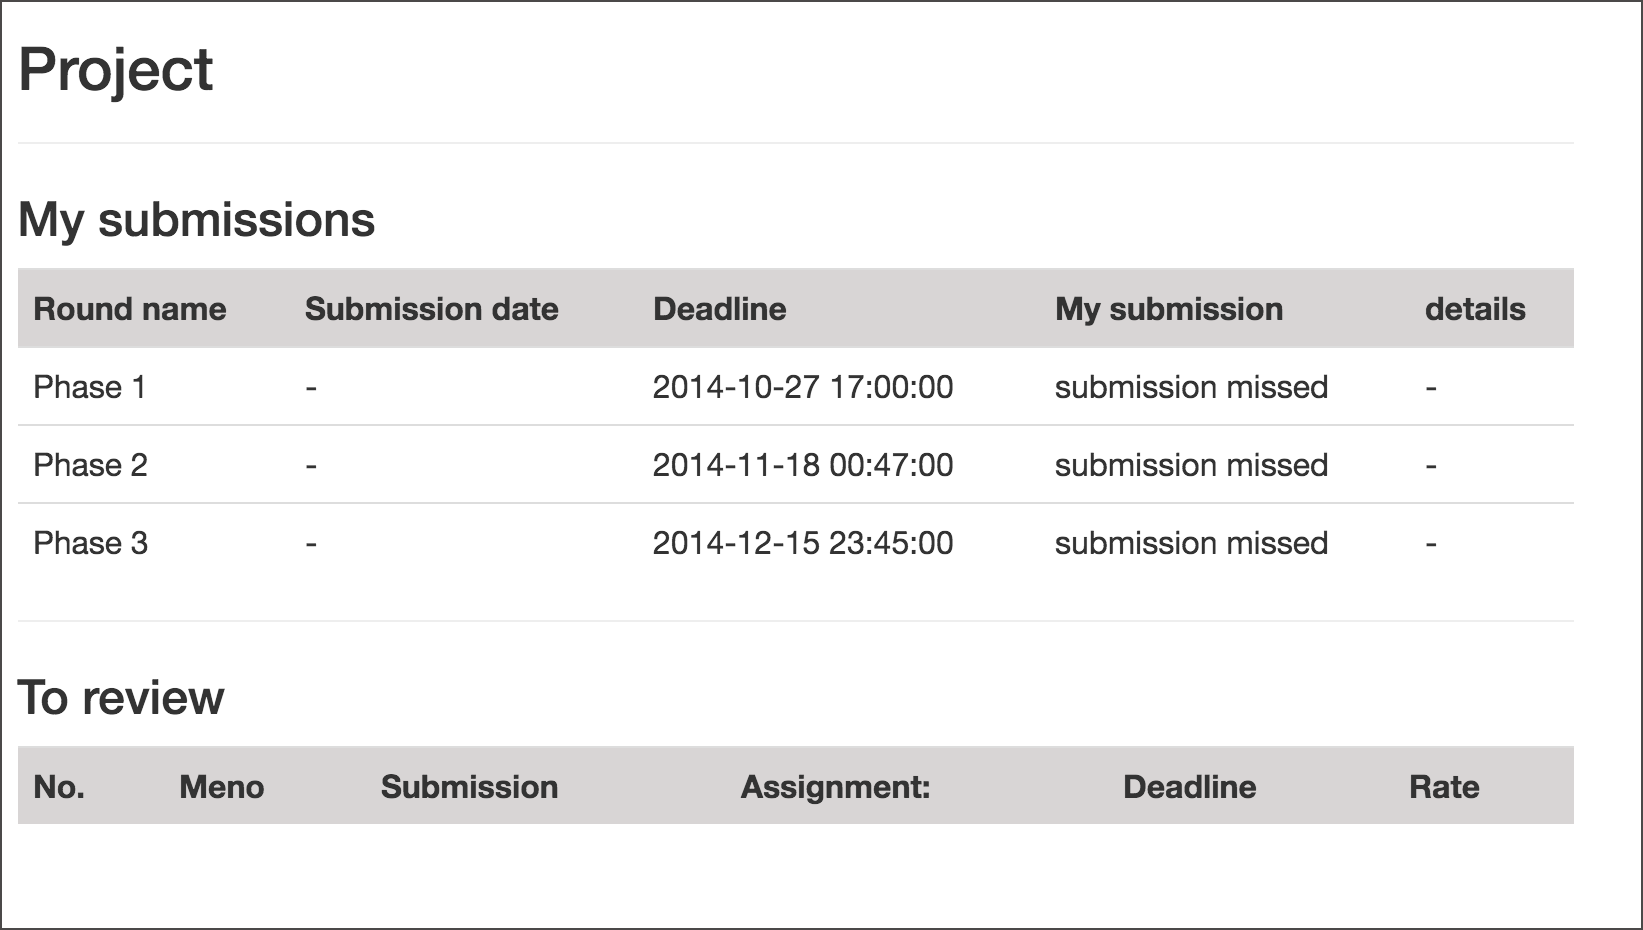
\includegraphics[width=0.95\textwidth]{images/assstudent.png}
    \caption{Student's part of assignment module}
    \label{assstudent}
\end{figure}


There are basicaly three possibilities: student can submit his homework assignment with added support for multiple assignment rounds. This means that each assignments can have multiple round, each of them can have different specifications. For example in first round, student must complete 50\% of selected tasks and in second round all of the tasks have to be completed. Second important functionality is reviewing of each round. After student submits a submission, other students can see it and write their feedback to this student. These feedback are often also evaluated and projected into final grade of the course. Thirth possibility is to view evaluations from teacher and classmates.

\subsection{Teacher's part}

This interface is way more complex. It offers multiple screens, some of them are presented on figure \ref{teachereval} and \ref{teacherrounds}. This interface also provides two important functionalities: assignment and review operations (create assignment, assign reviews on submitted assignments, delete assignment, edit assignment) and evaluation (assignments and reviews).



\begin{figure}[h]
    \centering
    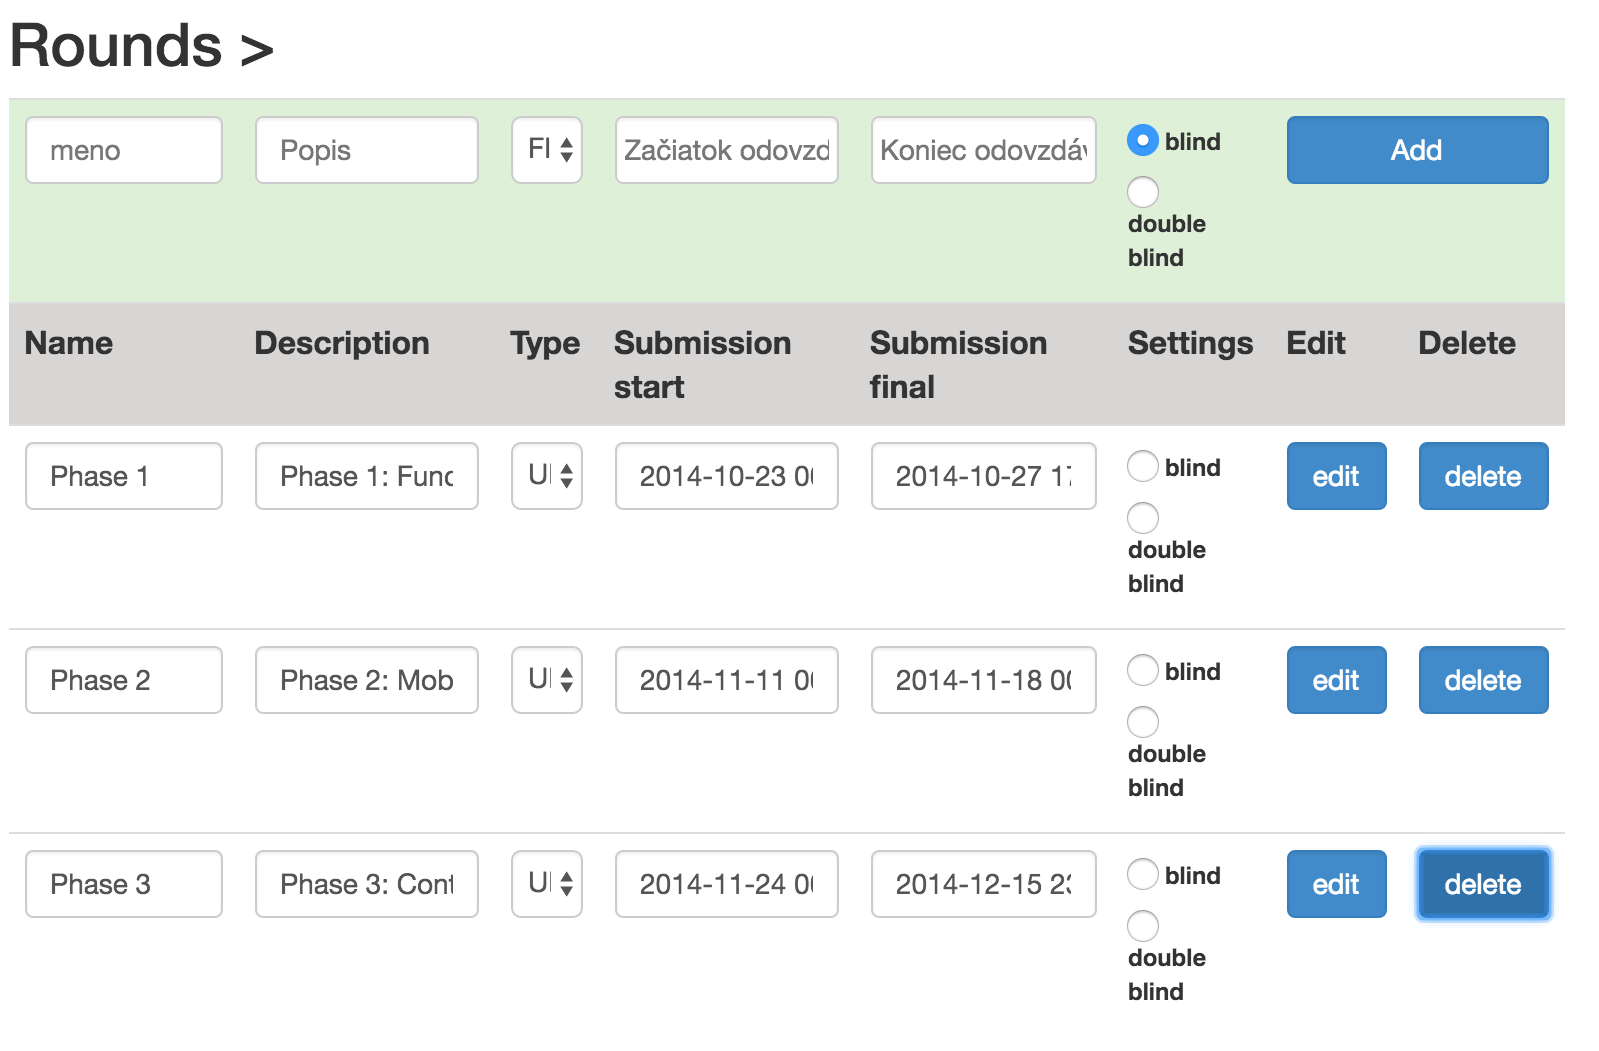
\includegraphics[width=0.95\textwidth]{images/teacherrounds.png}
    \caption{Teacher's administration of assignment rounds}
    \label{teacherrounds}
\end{figure}


On figure \ref{teacherrounds} is shown assignment round management. It is possible to set name of the assignment (to diferentiate multiple assignments), set it's description (which may provide some instructions for students), type (URL of FILE), submission deadlines and blindness settings. This system also allows double blind assignments. It is also possible to set student review deadlines, questions and ratings.

\begin{figure}[h]
    \centering
    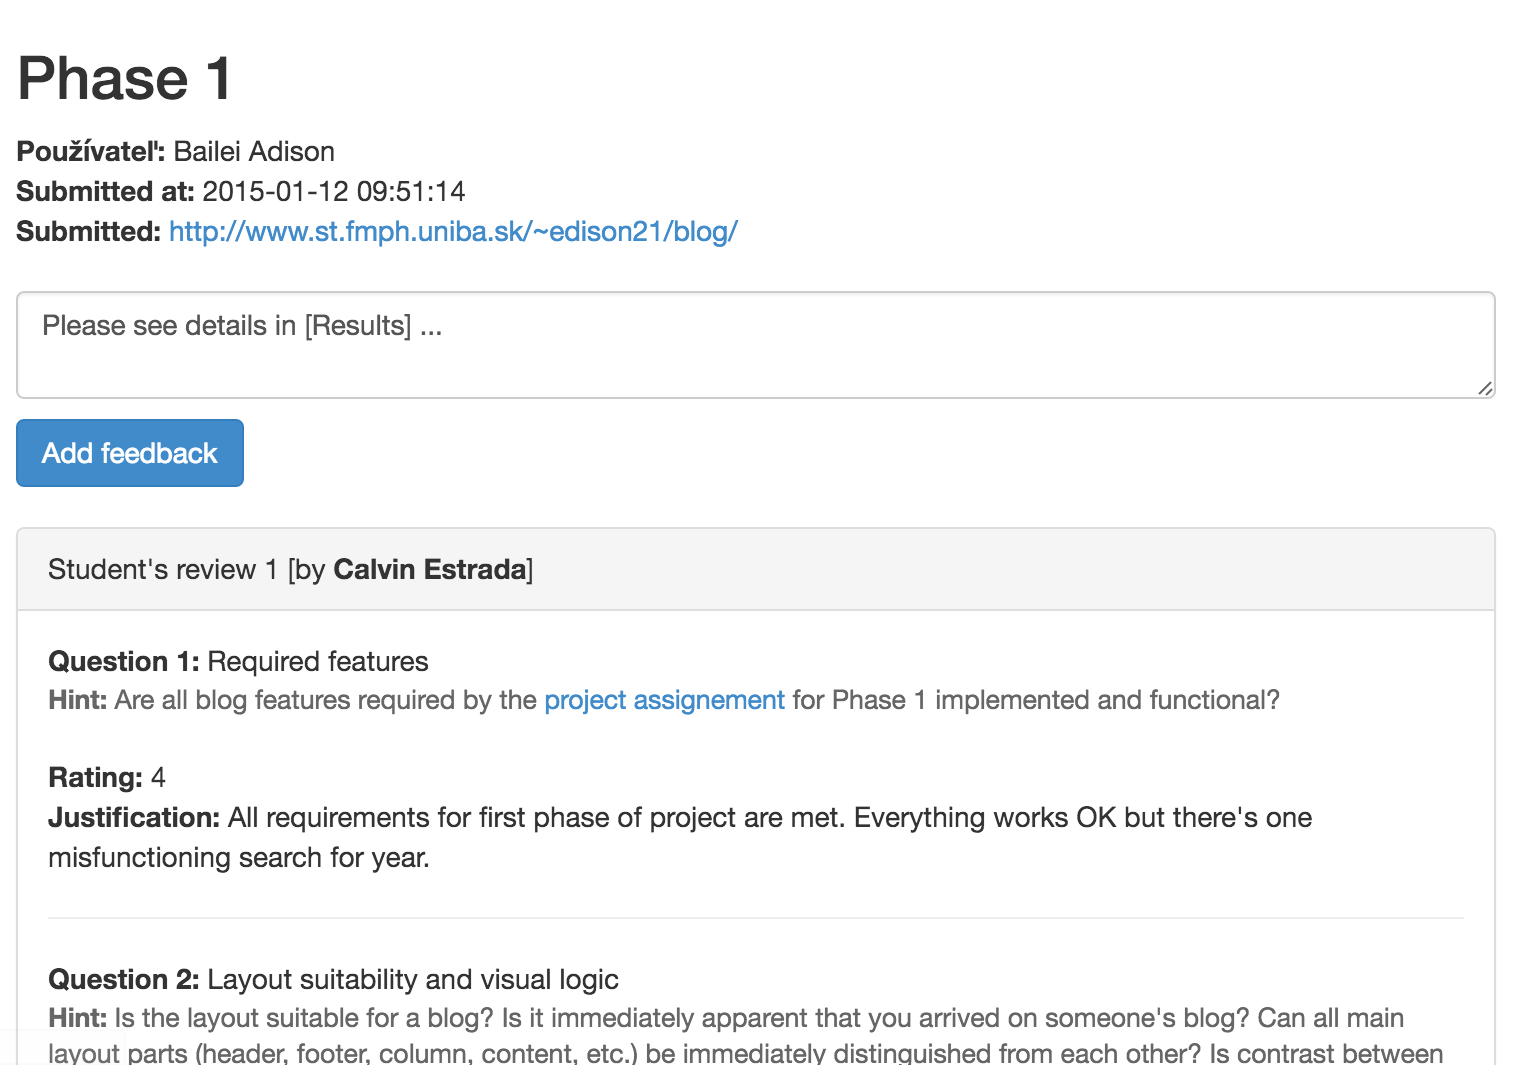
\includegraphics[width=0.95\textwidth]{images/teachereval.png}
    \caption{Teacher's evaluation of submitted assignments}
    \label{teachereval}
\end{figure}


On figure \ref{teachereval} we can see teacher's evaluation screen. Each round of an submitted assignment is presented on its own screen. The teacher is allowed to submit his own comment to this assignment and evaluate this assignment. There are also shown other student's reviews for this particular round of assignments. 

\section{Implementation}

Whole module is located in \texttt{application/modules/assignment} folder with file structure as described by CodeIgniter Modular Extensions. Now let's go through code flow of this module.


At first, as soon as system part of Courses 2 finds out that assignment module has to be run, routing of this module takes part. All routes are located in \texttt{application/modules/assignment/routes.php}. This script also loads correct course from database and acts as a "bootloader". After correct controller is decided from routing, it is instantiated and run.

\begin{lstlisting}[label={assrouting}, caption={Routing in assignments module for administrator}]
if (is_admin())
{
    switch (url_segment(3))
    {
        case false:
            $route['assignments'] = 'user/assignments';
            break;
        case 'admin':
            $route['assignments'] = 'admin/assignments';
            break;
        case 'reviews':
            $route['assignments'] = 'admin/manage_reviews';
            break;
        default:
            $route['assignments'] = 'admin/manage_assignments';
    }

    return;
}
\end{lstlisting}


After end of Jakub Culik's \cite{culik} work, there were 6 controllers in this module. 3 of them were used for teacher's administration and 3 were used for student's part. All controllers extend \texttt{Module\_Controller} class and implement \texttt{Module\_Interface}, which is special superclasses for all modules controllers. Otherwise they comply with standard development habbits.


Models are located in \texttt{application/modules/assignment/models/} and views in \texttt{application/modules/assignment/views}. As seen on \ref{assviews}, since there is none template engine used, views easily get pretty complicated. There's a lot of programming and scripting languages mixed together which can bring great chaos. On listing \ref{assviews} we can recognize HTML, PHP, PHP translations or even raw text mixed up together. We consider this a bad practice and propose usage of template engine system.

\begin{lstlisting}[label={assviews}, caption={Example of view in assignments module}]
<h2><?= lang('rating') ?>: <?= $submission['round_name'] ?></h2>
<br>
<b><?= lang('for_submission') ?>:</b> <a href="<?= $submission['submission'] ?>"><?= $submission['submission'] ?></a><br>
<b>By:</b> <?= $submission['user_name'] ?><br><br>
\end{lstlisting}
